\documentclass[rmp,10pt,onecolumn,fleqn,notitlepage]{revtex4-1}

\usepackage{graphicx}
\usepackage{color}
\usepackage{latexsym,amsmath}
\usepackage{physics}
\usepackage{tabularx}
\usepackage{float}
\usepackage{siunitx}
\usepackage{amssymb}

% Listing packages
\usepackage{xcolor}
\usepackage{listings}
\usepackage{framed}
\usepackage{inconsolata} % To change the listing font

% URL package and setting
\definecolor{linkcolor}{rgb}{0,0,0.65} %hyperlink
\usepackage[pdftex,colorlinks=true, pdfstartview=FitV, linkcolor= linkcolor, citecolor= linkcolor, urlcolor= linkcolor, hyperindex=true,hyperfigures=true]{hyperref} %hyperlink%

\usepackage{fancyhdr} % To change page setting

% PAGE SETTING
\pagestyle{fancyplain}
\fancyhf{}
\fancyfoot[R]{\thepage}
\fancyfoot[L]{\today}
\fancyhead[L]{\textbf{Week 4 Report, Quantum Information and Computing (2020)}}
\fancyhead[R]{\textbf{Alice Pagano}}
\renewcommand{\headrulewidth}{0.1pt}
\renewcommand{\footrulewidth}{0.1pt}

% LISTING SETTINGS
\definecolor{cadmiumred}{rgb}{0.89, 0.0, 0.13}
\definecolor{codegray}{rgb}{0.5,0.5,0.5}
\definecolor{commentcolour}{rgb}{0.43,0.63,0.65}
\definecolor{darkgreen}{rgb}{0.0, 0.5, 0.0}

\lstdefinestyle{Fortran}{language=Fortran,
    backgroundcolor=\color{white},
    commentstyle=\color{commentcolour},
    keywordstyle=\bfseries\color{cadmiumred},
    numberstyle=\tiny\color{codegray},
    stringstyle=\color{darkgreen},
    basicstyle=\ttfamily\footnotesize,
    breakatwhitespace=false,
    breaklines=true,
    captionpos=b,
    keepspaces=true,
    numbers=left,
    numbersep=5pt,
    showspaces=false,
    showstringspaces=false,
    showtabs=false,
    tabsize=2,
    frame=single,
    framexleftmargin=11pt,
    %rulecolor=\color{cadmiumred}
}
%\lstset{style=Fortran}

\lstdefinestyle{Gnuplot}{
    backgroundcolor=\color{white},
    commentstyle=\color{commentcolour},
    basicstyle=\ttfamily\footnotesize,
    breakatwhitespace=false,
    breaklines=true,
    captionpos=b,
    keepspaces=true,
    showspaces=false,
    showstringspaces=false,
    showtabs=false,
    tabsize=2
}

\lstdefinestyle{Python}{language=Python,
    backgroundcolor=\color{white},
    commentstyle=\color{commentcolour},
    keywordstyle=\color{darkgreen},
    numberstyle=\tiny\color{codegray},
    stringstyle=\color{cadmiumred},
    basicstyle=\ttfamily\footnotesize,
    breakatwhitespace=false,
    breaklines=true,
    captionpos=b,
    keepspaces=true,
    numbers=left,
    numbersep=5pt,
    showspaces=false,
    showstringspaces=false,
    showtabs=false,
    tabsize=2,
    frame=single,
    framexleftmargin=11pt
}

% BIBLIOGRAPHY FILE AND SETTING
\begin{filecontents*}{\jobname.bib}
    @article{cite1,
      title={Error handling in Fortran 2003},
      author={Koen Poppe and Ronald Cools and Bart Vandewoestyne},
      journal={ACM Sigplan Fortran Forum},
      year={2012},
      volume={31},
      pages={7-19}
    }
\end{filecontents*}

\bibliographystyle{aipnum4-1}
\setcitestyle{numbers,square}








\begin{document}



\title{Week 4: Multi-Run Script for Matrix-Matrix Multiplication}
\author{Alice Pagano}
\date{\today}

\begin{abstract}
In this Report, we analyze the computational time required by matrix-matrix multiplication for different multiplication methods. We use the modules implemented in the last two reports, in which we define a matrix type, user implemented algorithms for matrix-matrix multiplication with the adding of several control conditions to check if the operations are performed correctly. First of all, we create an input file with the matrix dimension \( N \), then a python script changes between the two values \( N_{min} \) and \( N_{max} \) and launches the program.  The results for the different multiplication methods are plotted in log-log scale and fitted with a straight line. The slope coefficient of the line define the order of the scaling.
\end{abstract}

\maketitle


\section{Theory}
In linear algebra, \textbf{matrix multiplication} is a binary operation that produces a matrix from two matrices.
If $A$ is an $m \times n$ matrix and $B$ is an $n \times p$ matrix:
\begin{equation}
    A =
  \begin{pmatrix}
     a_{11} & a_{12} & \dots  & a_{1n} \\
     a_{21} & a_{22} & \dots  & a_{2n} \\
     \vdots & \vdots & \ddots & \vdots \\
     a_{m1} & a_{m2} & \dots  & a_{mn}
  \end{pmatrix}, \qquad
  B =
\begin{pmatrix}
   b_{11} & b_{12} & \dots  & b_{1p} \\
   b_{21} & b_{22} & \dots  & b_{2p} \\
   \vdots & \vdots & \ddots & \vdots \\
   b_{n1} & b_{n2} & \dots  & b_{np}
\end{pmatrix}
\end{equation}
The matrix product $C = AB$ is defined to be the $m \times p$ matrix:
\begin{equation}
    C =
  \begin{pmatrix}
     c_{11} & c_{12} & \dots  & c_{1p} \\
     c_{21} & c_{22} & \dots  & c_{2p} \\
     \vdots & \vdots & \ddots & \vdots \\
     c_{m1} & c_{m2} & \dots  & c_{mp}
  \end{pmatrix}
\end{equation}
The product of matrices $A$ and $B$ is then denoted simply as \( C = AB \).


Matrix-matrix multiplication is a memory-bound computation because the reusage of memory is low.
If we consider the latency of a typical memory as less than 100 ns compared to the time required to perform a floating point operation (less than 1ns), we see that the majority of time is spent loading and storing values from/to arrays. We can implement an algorithm having data locality as much as possible: since the memory is loaded to the cache as lines, we have to use a loaded line of cache as much as possible, that is why accessing contiguous memory regions reduce the time spent loading data from memory.
In computing, \textbf{row-major order} and \textbf{column-major order} are methods for storing multidimensional arrays in linear storage such as random access memory.
The difference between the orders lies in which elements of an array are contiguous in memory. In row-major order, the consecutive elements of a row reside next to each other, whereas the same holds true for consecutive elements of a column in column-major order.
In Fortran, arrays are stored in \emph{column-major order}. In order to write a faster user implemented algorithm for matrix-matrix multiplication we have to take into account the memory order: the best choice is with the most inner loop which scan between rows.


In principle, the order of time scaling of the matrix multiplication algorithm is a power-law of the form:
\begin{equation}
  y (x) = k x^{n}
\end{equation}
We can take any relationship of this form, take the logarithm of both sides, and convert it to a linear relationship whose slope and intercept are related to the unknown values of $n$ and $k$:
\begin{equation}
  \log y = n \log x + \log k
\end{equation}
A graph that plots $\log y$ versus $\log x$ in order to linearize a power-law relationship is called a \textbf{log-log graph}.



\section{Code Development}

First of all, we create a python script “\texttt{input.py}” which define the input data, i.e. the matrix sizes for the multiplication. In particular, a list between two values \( N_{min} \) and \( N_{max} \) is created. In order to plot the data in log-log scale, we create a list of integers which are spaced evenly on a log scale.

Then, we develop three Fortran programs in which we perform matrix-matrix multiplication with different methods:
\begin{itemize}
\item in “\texttt{mat$\_$mul$\_$row.f90}”, we call \texttt{SUBROUTINE} {\bfseries\texttt{MatMultbyRow}}\texttt{(A,B,C)} in which the most inner loop of matrix multiplication scan between rows (accessing contiguous element in memory):

\begin{minipage}[t]{0.53\linewidth}%\vspace{0pt}
\begin{lstlisting}[style=Fortran]
do jj=1,p
    do kk=1,n
        do ii=1,m
            C(ii,jj) = A(ii,kk) * B(kk,jj) + C(ii,jj)
        end do
    end do
end do\end{lstlisting}
\end{minipage}

\item in “\texttt{mat$\_$mul$\_$col.f90}”, we call \texttt{SUBROUTINE} {\bfseries\texttt{MatMultbyCol}}\texttt{(A,B,C)} in which the second loop of matrix multiplication scan between columns (in any case, we are not accessing contiguous element in memory):

\begin{minipage}[t]{0.53\linewidth}%\vspace{0pt}
\begin{lstlisting}[style=Fortran]
do ii=1,m
    do jj=1,p
        do kk=1,n
            C(ii,jj) = A(ii,kk) * B(kk,jj) + C(ii,jj)
        end do
    end do
end do\end{lstlisting}
\end{minipage}

\item in “\texttt{mat$\_$mul$\_$mat.f90}”, we call the standard \texttt{FUNCTION} {\bfseries\texttt{MatMul}}\texttt{(A,B)}.

\end{itemize}

Each file takes as input the matrix dimension $N$ and the name of the file in which the output will be written. Then, matrix \( A \) and \( B \) are randomly initialized, while matrix \( C \) is initialized to zero. After that, matrix multiplication is performed for 6 times and each time the computational time is registered. We compute the average time (without the first time of each execution) with the corresponding standard deviation and we print them in a file.

After that, we develop a python script “\texttt{script.py}” which, in order:
\begin{itemize}
\item load the input data and clean older executable files and results;
\item compile the three programs for different optimization flags: -O0, -O1, -O2 and -O3;
\item for each flag, we iterate for the input values of matrix size and for each size we call the three different executable “\texttt{mat$\_$mul$\_$row}”, “\texttt{mat$\_$mul$\_$col}” and “\texttt{mat$\_$mul$\_$mat}”;
\item after that, for each optimization flag, the results for the three different method are plotted in log-log scale with the corresponding linear fit using a gnuplot script “\texttt{fit.p}”.
\end{itemize}

\begin{minipage}[t]{0.73\linewidth}%\vspace{0pt}
\begin{lstlisting}[style=Python]
executable = ['mat_mult_row','mat_mult_col','mat_mult_mat']
optimization = ['O0','O1','O2','O3']

# Compile program for different optimization flags
for opt in optimization:
    make_command = ["make","all","FAST=-"+opt]
    make_proc = subprocess.run(make_command)
    # Iterate for values of matrix size
    for n in input_data:
            # Call executables
            for exe in executable:
                subprocess.run(['./'+exe,str(n),'time_'+opt+'_'+exe+'.dat'])

# Plot fit for different optimization flags
for opt in optimization:
    subprocess.run(['gnuplot','-e',"opt_flag='"+opt+"'",'fit.p'])\end{lstlisting}
\end{minipage}



\section{Results}
We run the python scripts for \( N_{min}=100 \) and \( N_{max}=1500 \). The results for the different optimization flags are plotted in Fig. \ref{fig:results}. We note that for all the three methods the order of scaling is almostly as expected, i.e. \( O(N^3) \).

If no optimization flag is used (-O0 case), we note that the times required by the user-implemented algorithms are very high with respect to {\bfseries\texttt{MatMul}} function. So, in this plot the curves of {\bfseries\texttt{MatMultbyRow}} and {\bfseries\texttt{MatMultbyCol}} overlap and we cannot appreciate the difference in speed in accessing the elements by rows or by columns.
If we use the optimization flag -O1, the user-implemented algorthms speed-up and we start to see the difference between them. We note also that the optimization flag has no impact in the already optimized function {\bfseries\texttt{MatMul}}.
Increasing further the level of optimization to -O2 and -O3, we note a non relevant optimization for the user-implemented functions. The only thing to notice is that the difference in time between {\bfseries\texttt{MatMultbyRow}} and {\bfseries\texttt{MatMultbyCol}} starts to decrease.

We can conclude that the user-implemented functions are very slow and inefficient compared to the optimized standard function {\bfseries\texttt{MatMul}}. This is why the maximum matrix size that can be computed in a reasonable time is \( N_{max}=1500 \).


\begin{figure}[t!]
\begin{minipage}[c]{0.49\linewidth}
\centering
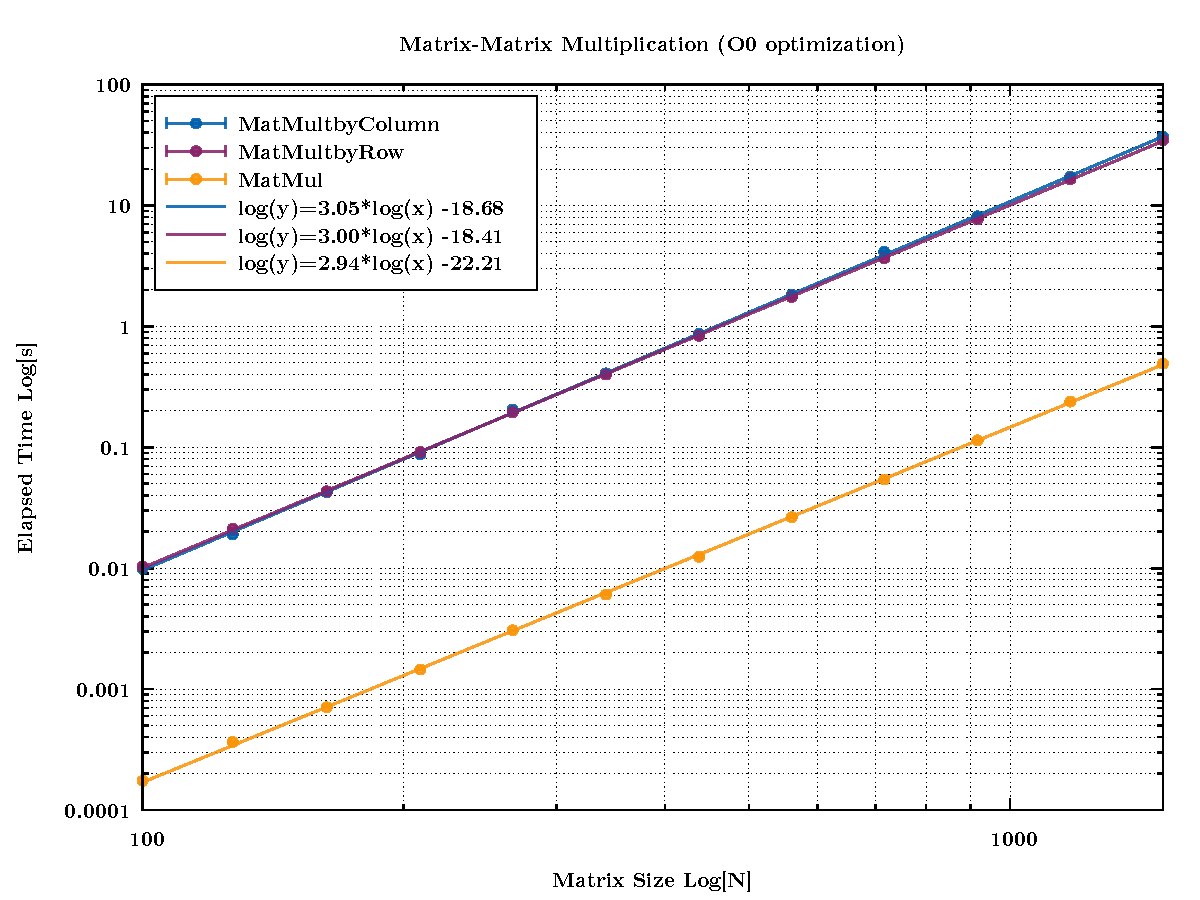
\includegraphics[width=1\textwidth]{image/matmult_O0.pdf}
\end{minipage}
\begin{minipage}[]{0.5\linewidth}
\centering
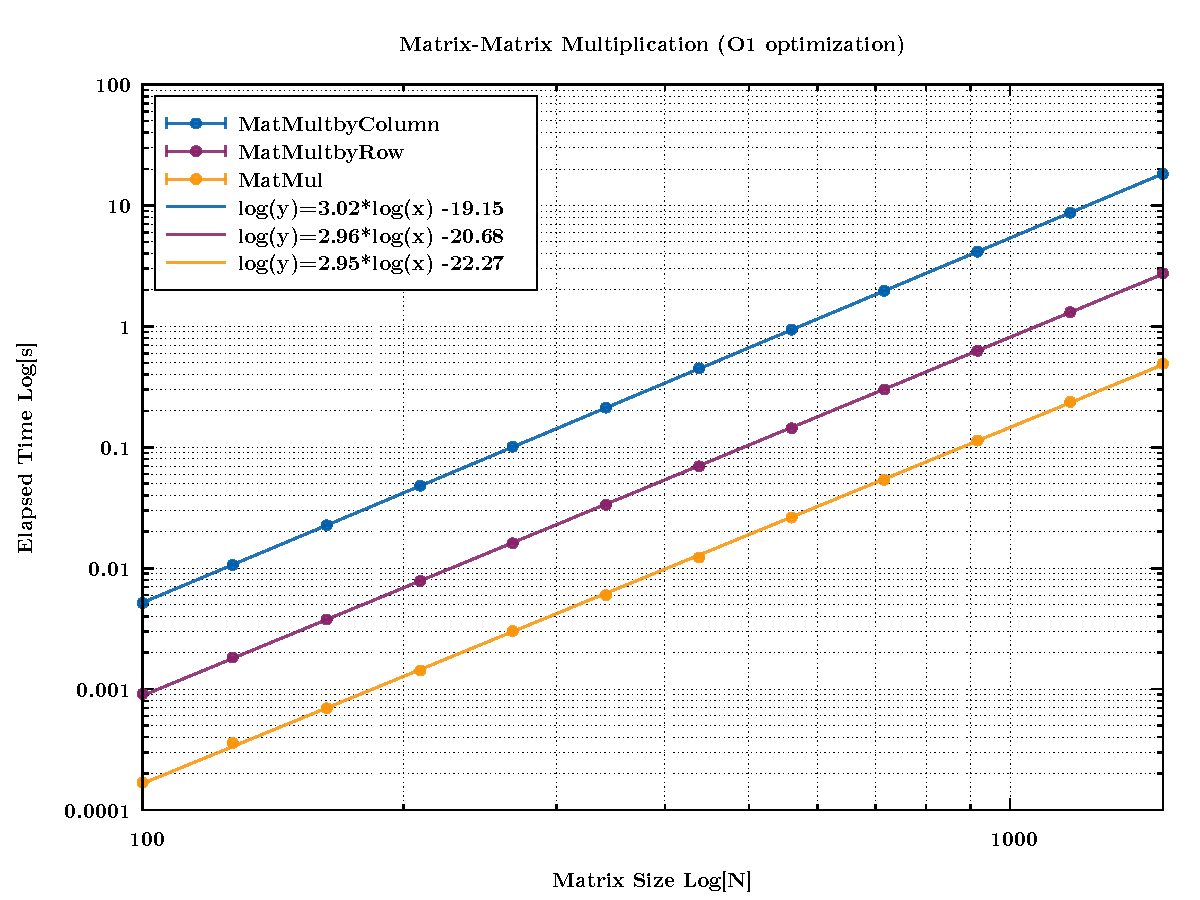
\includegraphics[width=1\textwidth]{image/matmult_O1.pdf}
\end{minipage} \\
\begin{minipage}[c]{0.49\linewidth}
\centering
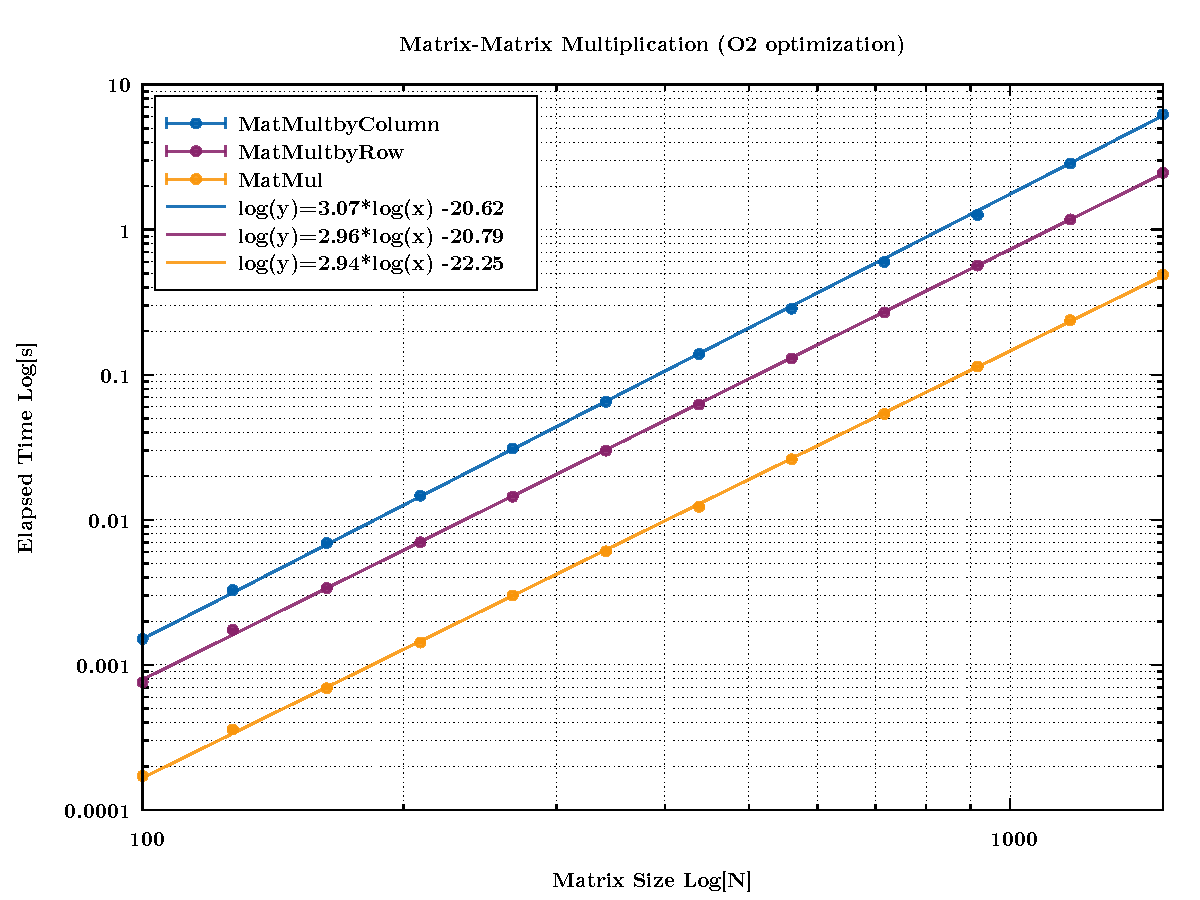
\includegraphics[width=1\textwidth]{image/matmult_O2.pdf}
\end{minipage}
\begin{minipage}[]{0.5\linewidth}
\centering
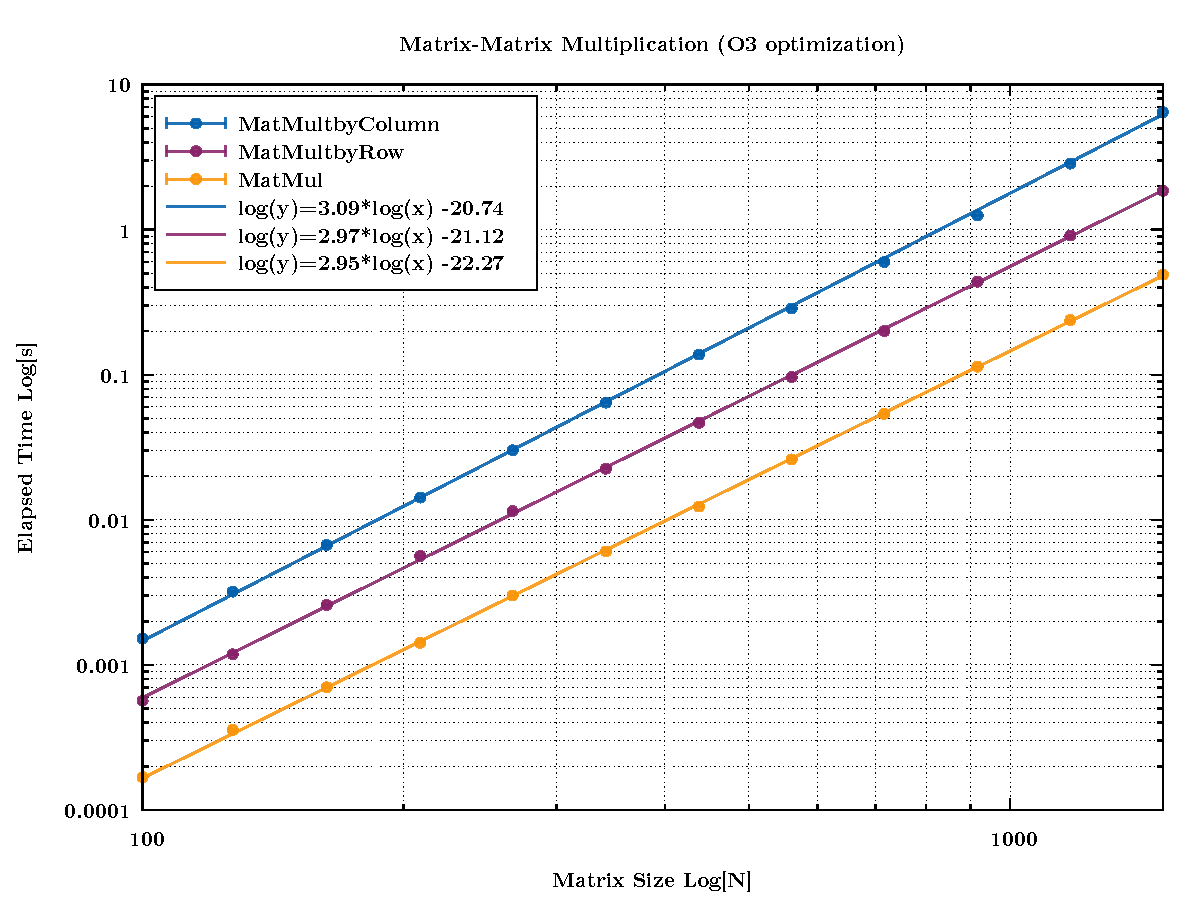
\includegraphics[width=1\textwidth]{image/matmult_O3.pdf}
\end{minipage}
\caption{\label{fig:results} Plots of computational time required by the three different multiplication methods for different optimization flags.}
\end{figure}


\section{Self-Evaluation}
In a further development of the matrix multiplication code, it would be efficient computing the matrix elements in batch by using different CPUs. This is what is probably already implemented in standard functions. An even better optimization would be parallelize the computation on GPUs.


% include bibliography
%\bibliography{\jobname}


\end{document}
